\documentclass[11pt,bibtotoc,noliststotoc,BCOR0mm]{scrbook}

% Codificación
\usepackage[spanish]{babel}
\usepackage[utf8x]{inputenc}

% Fuentes
\usepackage{lmodern}
\usepackage[T1]{fontenc}
\usepackage{textcomp}
\usepackage{parskip}

% Formato de página
\usepackage[a4paper]{geometry}
\geometry{verbose,lmargin=3.5cm,rmargin=2.5cm}
\usepackage[ilines]{scrpage2}

% Otros paquetes
\usepackage{tabularx}
\usepackage{array}
\usepackage{xspace}
\usepackage{varioref}
\usepackage{microtype}
\usepackage{tikz}
\usepackage{verbatim}
\usetikzlibrary{trees}

% hyperref casi siempre es mejor cargarlo al final
\usepackage[colorlinks,citecolor=blue]{hyperref}

\setheadsepline{.4pt}

\subject{Seguridad en los Sistemas Informáticos \\ 
   Departamento de Ingeniería Informática \\
   Universidad de Cádiz \\ Curso 2017/2018}
\title{Política de Seguridad Aseguradora de vida LifeSecur}
\author{
	\textbf{Grupo 8:}\\
    José Joaquín Arias Gómez-Calcerrada\\
	Manuel Diaz Gil\\
	Daniel Mejias Ramirez\\
	Jesús Rosa Bilbao\\
}
\date{\today}

\makeatletter
\hypersetup{
  pdftitle={Pol\'{i}tica de seguridad Aseguradora de vida LifeSecur}, 
  pdfsubject={Seguridad en los Sistemas Informáticos},
  pdfauthor={José Joaquín Arias Gómez-Calcerrada, Manuel Diaz Gil, Daniel Mejias Ramirez, Jesús Rosa Bilbao
},
  pdfkeywords={seguridad, pol\'{i}tica, tecnolog\'{i}as, informaci\'{o}n, inform\'{a}tica}
}
\makeatother

\newcommand{\cellcenter}[1]{\multicolumn{1}{c}{#1}}
\newcommand{\thead}[1]{\textbf{\emph{#1}}}
\newcommand{\espaciocambios}{\rule{0cm}{1.5cm}\xspace}
\setlength{\extrarowheight}{4pt}

\AtBeginDocument{
   \renewcommand{\tablename}{Tabla}
   \renewcommand{\listtablename}{Índice de tablas}
}

\begin{document}

% Portada
\begin{titlepage}
  \maketitle
\end{titlepage}

\frontmatter
\pagestyle{empty}

\tableofcontents
\listoffigures
\listoftables


\chapter{Historial de cambios}

\begin{center}
  \centering
  \begin{tabular}{|m{.2\textwidth}|m{.3\textwidth}|m{.4\textwidth}|}
    \cellcenter{\thead{Versión}} & \cellcenter{\thead{Fecha}} & \cellcenter{\thead{Descripción}} \\
    \hline
    1.0 & \today & Primera versión del documento. \\ \hline
    & &  \\ \hline
    & &  \\ \hline
    & &  \\ \hline
    & &  \\ \hline
  \end{tabular}
\end{center}


\chapter{Compromiso de la Dirección}

En este capítulo (no numerado) se escribirá una carta formal firmada y
sellada por los miembros relevantes de la dirección de la compañía y
por el Responsable de Seguridad, en la que se relaciona la seguridad
con las metas de la organización, se valida la versión actual de la
política y se compromete a proveer los recursos necesarios para su
ejecución.


\chapter{Aprobación y entrada en vigor}

Se indicará cuándo se ha aprobado el documento así como la fecha de entrada 
en vigor. 

\mainmatter
\pagestyle{scrheadings}


\chapter{Introducción} 

En este capítulo se hará una introducción a los aspectos fundamentales de nuetra organización, LifeSecur.

\section{Descripción de la organización}

LifeSecur es una organización que se dedicará a los seguros de vida para caso de muerte, es decir, para los seguros de vida riesgo.

\subsection{Objetivos de la organización}

Los objetivos principales de LifeSecur son proporcionar la suma asegurada, ya se trate de un capital o de una renta, si se produce la muerte del asegurado.

Nuestra organización pretende conseguir la mejor atención al cliente posible, además de garantizar que nuestros beneficiarios tengan suficiente dinero para mantener su estilo de vida.

LifeSecur exigirá los requisitos necesarios para dar un préstamo comercial.

\subsection{Descripción del edificio}

El conjunto consta de un único edificio. Éste será el edificio principal y en el que se realizarán todas las operaciones. Su sede se situará en Cádiz, concretamente en Puerto Real:

\textit{\textbf{Localización:}}\\
Calle Ribera del Muelle, 82\\
11510 Puerto Real(CA)

También se dispone de parking subterráneo para el personal autorizado (trabajadores de la empresa) y para el cliente, para facilitar el acceso a las instalaciones.

El edificio está compuesto en su mayor parte de oficinas para los trabajadores. También tendrá una zona de recepción al cliente y zonas de espera.

El acceso principal al edificio tendrá lugar desde la fachada orientada al norte del mismo. A la entrada del edificio se encontrará una zona de espera, junto a la cual se situará la zona de recepción al cliente y los aseos públicos.

El edificio principal consta de tres plantas principales, además de dos plantas subterráneas para los aparcamientos:

\textbf{Planta 1}

La zona de recepción al cliente se encuentra en frente de la entrada principal del edificio. Justo a su izquierda, se situa la primera zona de aseos. A la derecha de la zona de recepción se encuentra la zona de espera, compuesta por dos habitaciones contiguas y con asientos, mesas y revistas para pasar el tiempo muerto.

La habitación de comunicaciones, en la cual se encuentra el rack de planta y de edificio, se situa detrás de la zona de recepción. Justo a su derecha, se encuentran los aseos para el personal autorizado.

\textbf{Planta 2}

Desde el vestíbulo de la primera planta, se accede a las escaleras que le llevarán al vestíbulo de la segunda planta. A su derecha se sitúa el acceso a las oficinas del edificio, además de los departamentos de administración, seguridad e informática. Al final del pasillo principal de esta planta se encuentran las escaleras para acceder a la tercera planta.

\textbf{Planta 3}

Esta planta se encuentra ocupada por completo de ofinicas. Se puede acceder a la tercera planta por las escaleras o por el ascensor del edificio.

\textbf{Planta subterránea 1 y 2}

Estas plantas están ocupadas por los aparcamientos del edificio. Dispone de ascensor y escaleras para acceder a la planta 1.

\subsection{Organigrama de la organización}

\begin{tikzpicture}[
  man/.style={rectangle,draw,fill=white!20},
  grandchild/.style={grow=down,xshift=1em,anchor=west,
    edge from parent path={(\tikzparentnode.south) |- (\tikzchildnode.west)}},
  first/.style={level distance=6ex},
  second/.style={level distance=12ex},
  third/.style={level distance=18ex},
  level 1/.style={sibling distance=15em}]
    % Parents
    \coordinate
      child[grow=down,level distance=0ex] {node[man,anchor=west]{Presidente}}
    [edge from parent fork down]
    % Children and grandchildren
    child{node[man] {Responsable de Seguridad}
      child{node[man] {Departamento de Seguridad}
      	child{node[man] {Área Médica}}
        child{node[man] {Área de Comunicaciones}}
        child{node[man] {Área de Mantenimiento}}}}
    child{node[man] {Vicepresidente}};
\end{tikzpicture}
\\
\title{Figura 1: Organigrama de LifeSecur}

\newpage

\textbf{Presidente}

Ejerce la representación legal de la empresa. LifeSecur se regirá bajo la figura del presidente.

\textbf{Vicepresidente}

Trabaja como asistente principal del presidente. Realizará las tareas del presidente en su ausencia.

\textbf{Responsable de Seguridad}

Persona o personas con función de coordinar las medidas de seguridad aplicables. A este se le deben comunicar todas las incidencias que puedan afectar a la seguridad de los ficheros con datos personales.

\textbf{Departamento de Seguridad}

Departamento encargado de la seguridad de la empresa. Consta de varias áreas: Área Médica, área de comunicaciones y área de mantenimiento.

\textbf{Área Médica}

Departamento encargado de todo lo relacionado con los activos orgánicos. Abarca desde su manipulación, seguido por la recogida de los donantes, hasta su traslado al edificio principal.

\textbf{Área de Comunicaciones}

Departamento encargado de la administración de todo lo que engloba el equipo de comunicaciones. El objetivo principal es el de manejar y transmitir la información de forma óptima.

\textbf{Área de Mantenimiento}

Departamento encargado del mantenimiento de los activos de la empresa, como la parte informática, mecánica y limpieza.

\section{Objetivos y alcance de la política}

El objetivo principal de esta política de seguridad es la de dotar de un nivel alto de seguridad a todas las áreas del edificio. Para esto es imprescindible que estén actualizadas, para protegerse de cualquier tipo de amenaza externa. Por ejemplo, los activos orgánicos del área médica son muy sensibles a estas posibles amenazas externas.

\section{Gestión de cambios de la política}

La política de seguridad será actualizada cada trimestre. En cada uno, se realizarán reuniones compuestas por el presidente, el vicepresidente y el director del departamento de seguridad.

Las reuniones se compondrán de una recopilación de los cambios recopilados a actualizar y una puesta en común para aprobarlos y/o mejorarlos.

Para ello, las propuestas de los cambios de la política de seguridad deben ser almacenadas en un fichero protegido. Estas propuestas podrán llegar de todos los departamentos y de los empleados de LifeSecur.

La política de seguridad sólo se actualizará cuando sea aprobada. Entonces, se establecerá y hará pública  vía e-mail una fecha para su entrada en vigor.

Para las proposiciones de cambios se debe rellenar un formulario de solicitud de cambio, establecido en el Anexo C.

\section{Organización de la seguridad}

El jefe del departamento de seguridad será el encargado de asegurar que las normas, leyes, reglas y principios especificados en la política de seguridad se cumplen.

El jefe del departamento de seguridad será también el encargado de informar sobre las posibles incidencias ocurridas.

Cada año, se realizarán cursos a los empleados para recordar la aplicación de las normas de la política de seguridad.

\chapter{Política de seguridad de la información}

\section{Ámbito}

Esta política se aplica a todo el personal de la empresa LifeSecur y también al personal subcontratado, es decir, que trabaje para una empresa que esta a su vez trabaje para LifeSecur, que trabaje con los datos de la empresa LifeSecur.


\section{Objetivos}

LifeSecur tiene propuesto una serie de objetivos con el fin de asegurar el cumplimento de la integridad, no repudio, legalidad y confidencialidad.

	- Mantener la confianza de los ciudadanos respecto al manejo y protección de la información que utilizada en LifeSecur.
    
	- Cumplir los principios de la seguridad de la información: Disponibilidad, integridad y confidencialidad.
    
	- Proteger los recursos de información de LifeSecur y la tecnología utilizada frente amenazas tanto interna como externa, ya sea causas humanas como naturales.
    
	- Asegurar la implementación de medidas de seguridad propuesta en esta Política.
    
	- Mantener la política de LifeSecur actualizada, para poder asegurar su vigencia y eficacia.


\section{Alcance y responsabilidades}

Esta política se aplica a todo el ámbito de LifeSecur, ya sean recursos, procesos, sus funcionarios, contratistas externo o interno y cualquier empleado de LifeSecur que tengan acceso a la información, infraestructura tecnológica, equipos y canales de comunicación.

El director del departamento de informática será el encargado de tener el rol de responsable de la seguridad de LifeSecur. Teniendo por funciones:

	- Mantener la seguridad de la información.
    
	- Realizar o promover la auditorias que permitan conocer el grado de cumplimiento de la empresa en el tema de la política de seguridad.
    
	- Analizar y aprobar toda la documentación de relacionada con la seguridad.
    
	- Supervisar cualquier incidente relacionado con la seguridad.


\section{Información recogida}

La empresa LifeSecur recogerá la información relacionada a los datos personales de los clientes, su historial clínico y su cuenta bancaria.
Los datos personales como son el teléfono, dirección, DNI, nombre y apellidos serán recogidos para poder identificar a cada cliente y facilitar su contacto en el caso de comunicación por parte de la empresa.

Historial Clínico forma parte de la lógica de negocio de nuestra empresa ya que historial clínico influye directamente en el seguro entre nuestra empresa y el cliente.

Cuenta bancaria es un dato necesario para nuestra empresa ya que los pagos mensuales se harán de manera única y exclusiva median transacciones bancarias.


\section{Análisis de riesgos y sensibilidad}

Historial clínico es una información muy delicada de alta seguridad según las leyes de protección de datos, que no debe ser susceptible de ser manipulada por alguien ajeno al responsable de dicha manipulación de información.

Datos Bancarios que según la ley actual de protección de datos forma parte de los datos de nivel medio, y que la manipulación de manera inapropiada tendría una consecuencia directa en el cliente al cual le pertenecen dichos datos.

Posibles riesgos pueden correr estas informaciones:

	- Denegación de servicio: con este ataque impedirían el acceso a la información por lo que no se cumpliría una de las bases de la seguridad, la disponibilidad.
    
	- Ataque a la información tanto desde el interior como del exterior: esto afectaría a la integridad y confidencialidad de los datos clínico.
    
	- Eliminación del archivo por fallo humano: este fallo pondría en riesgo todas las bases de la seguridad.
    
	-Revelación de la información: Acción que pondría en riesgo la confidencialidad de los datos.


\subsection{Activos}
Se detallarán los activos de información de la organización. 
La información es un activo abstracto que será almacenado en 
equipos o soportes de información (normalmente agrupado como ficheros o bases 
de datos) o será transferido de un lugar a otro por los medios de 
transmisión de datos. 

A continuación vamos a enumerar los distintos activos de información que vamos a tratar en nuestra organización el orden de importancia sera de mayor a menor segun la posición que ocupen en la lista:
\begin{itemize}
\item Expedientes medicos
\item Partes/Siniestros
\item Datos bancarios
\item Datos personales
\end{itemize}
Toda esta información estará almacenada en una base de datos específicamente para este fin, que sea lo mas segura posible cumpliendo varios protocolos de seguridad, aparte se mantendra una copia local de todos estos datos en discos locales cifrados en unos armarios especializados anti robo e ignifugos.

\subsection{Amenazas sobre los activos}
Se especificarán las amenazas a las que se verá sometida la información de 
la empresa, y su valoración en base a la confidencialidad, integridad y 
disponibilidad:

\textbf{[PSI] Política de seguridad de la información}
\begin{center}
  \centering
  \begin{tabular}{|m{.2\textwidth}|m{.2\textwidth}|m{.2\textwidth}|m{.2\textwidth}|m{.2\textwidth}|}
    \cellcenter{\thead{Valoración}} & \cellcenter{\thead{Enumeración}} & \cellcenter{\thead{Activo}} 
& \cellcenter{\thead{Amenazas}} & \cellcenter{\thead{Dimensiones}} \\ \hline
    9 (o muy alta) & PSI.1, PSI.2 ... & [source] & E.1, E.2... & [I] \\ \hline
    9 & 9.PSI & Expedientes medicos & Robo, inundaciones, incendios, exploit, phishing & [I] \\ \hline
      & 9.PSI2 & Partes/Siniestros & Robo, inundaciones, incendios, exploit, phishing & [I] \\ \hline
    7 & 7.PSI & Datos bancarios & Robo, inundaciones, incendios, exploit, phishing & [I] \\ \hline
    5 & 5.PSI & Datos personales & Robo, inundaciones, incendios, exploit, phishing & [I] \\ \hline
  \end{tabular}
\end{center}

\section{Conformidad con la legislación vigente}

Nuestra politica de seguridad debe cumplir y cumplirá las siguientes leyes sobre protección de datos, que regula tanto el ambito físico como electrónico de la trata de datos personales de todos nuestros clientes:
\begin{itemize}
\item LO15/1999
\item L59/2003
\item RD1720/2007
\item RD3/2010
\item RGPD 2016/679
\end{itemize}
Vamos a integrar todas estas leyes en nuestra empresa de diferentes maneras, en primer lugar cuando se recaben los datos de los clientes ya sea de forma fisica y/o electronica, se le informara en todo momento de:
\begin{itemize}
\item De que esos datos se van a almacenar en un fichero, que puede ser posteriomente tratado.
\item De la finalidad para la que se recogen los datos y el destinatario de la información.
\item Del carácter obligatorio o no de su respuesta a las preguntas que se le hacen.
\item De las consecuencias de la obtención de los datos o de la negativa a suministrarlos.
\item De la posibilidad de ejercer su derecho de acceso, recticación,cancelación y oposición.
\item De la identidad y dirección del responsable del tratamiento, o en su caso de su representante
\end{itemize}
En segundo lugar, a parte de informar en todo momento a los clientes de todo lo mencionado anteriormente tambien tienen una serie de derechos a los que pueden acudir en cualquier momento:
\begin{itemize}
\item Derecho al olvido: Los ciudadanos tienen derecho a solicitar, y obtener de los responsables, que los datos personales sean suprimidos cuando estos ya no sean necesarios para la nalidad con la que fueron recogidos
\item Derecho a la portabilidad: Implica que el interesado que haya proporcionado sus datos a un responsable que los esté tratando de modo automatizado podrá solicitar recuperar esos datos en un formato que le permita su traslado a otro responsable.
\end{itemize}
Toda esta información se proporcionara en un lenguaje claro y conciso de forma que sea facil de entender para cualquier usuario y se revisaran los sistemas de registro para verificar el consentimiento de todos los usuarios de forma que se pueda verificar dicho consentimiento ante una posible auditoria.

\chapter{Política de seguridad física}
\label{ch:fisica}

\section{Ámbito}

Cuando hablamos de seguridad física nos referimos a todos aquellos mecanismos generalmente de prevención y detección destinados a proteger físicamente cualquier recurso del sistema; estos recursos son desde un simple teclado hasta una copia de seguridad con toda la información que hay en el sistema.

Dependiendo del entorno y los sistemas a proteger esta seguridad será más o menos importante y restrictiva, aunque siempre deberemos tenerla en cuenta.

El hardware es frecuentemente el elemento más caro de todo sistema informático y por tanto las medidas encaminadas a asegurar su integridad son una parte importante de la seguridad física de cualquier organización.
\begin{itemize}
\item Acceso físico
\item Desastres naturales
\item Alteraciones del entorno
\end{itemize}

Además proteger el hardware nuestra política de seguridad debe incluir medidas de protección de los datos, ya que en realidad la mayoría de ataques tienen como objetivo la obtención de información, no la destrucción del medio físico que la contiene.
\begin{itemize}
\item Eavesdropping o interceptación
\item Copias de seguridad
\item Soportes no electrónicos
\end{itemize}

\section{Objetivos}

La gran cantidad de nuestros datos estaran informatizados, estando el mayor riesgo en el acceso a cualquier equipo fisico situado en la empresa mas que en los propios papeles por lo que vamos a enumerar los distintos objetivos que pretendemos alcanzar con nuestra politica de seguridad fisica:
\begin{itemize}
\item Protección de recursos: El esquema de protección de recursos garantiza que solo los usuarios autorizados podrán acceder a los objetos del sistema.Definiendo con precisión las distintas categorías de usuarios que pueden acceder al sistema. Asimismo, qué tipo de autorización de acceso se otorga a estos grupos de usuarios.
\item Autenticación: Hacer uso de los certificados digitales para ofrecer un método más seguro de autenticación, a la vez que proporcionan otras ventajas de seguridad. Buscando ofrecer un nivel mas de seguridad que lo tradicionalmente usado de usuario y contraseña. Los usuarios autenticados podrían tendran distintos tipos de permisos, según su nivel de autorización.
\item Autorización: Seguridad de que la persona o el sistema situado en el otro extremo de la sesión tiene permiso para llevar a cabo la petición. La autorización es el proceso de determinar quién o qué puede acceder a los recursos del sistema o ejecutar determinadas actividades en un sistema. La autorización se realizara en el contexto de la autenticación.
\item Integridad: Seguridad de que la información entrante es la misma que la que se ha enviado.

\item Integridad de los datos: los datos están protegidos contra cambios o manipulaciones no autorizados.Protegiendolos para que no se puedan husmear ni interpretar, lo que se hara cifrándolos.
\item No repudio: Prueba de que se ha producido una transacción o de que se ha enviado o recibido un mensaje. Se usaran certificados digitales y criptografía de claves públicas para firmar transacciones, mensajes y documentos siendo esta la base del no repudio.
\item Confidencialidad: Es la seguridad de que la información confidencial permanece privada y no es visible para los escuchas intrusos. La confidencialidad es fundamental para la seguridad total de los datos. El cifrado de los datos con certificados digitales y la capa de sockets segura (SSL) o con una conexión de redes privadas virtuales (VPN) nos permitira asegurar la confidencialidad al transmitir datos entre varias redes que no sean de confianza.
\item Actividades de seguridad de auditoría: Consisten en supervisar los eventos relacionados con la seguridad para proporcionar un archivo de anotaciones de los accesos satisfactorios y de los no satisfactorios (denegados). Los registros de accesos satisfactorios indican quién está haciendo cada tarea en los sistemas. Los registros de accesos no satisfactorios (denegados) indican que alguien está intentando abrirse paso a través de las barreras de seguridad del sistema o que alguien tiene dificultades para acceder al sistema.

\end{itemize}

\section{Alcance y responsabilidades}
Esta política se aplica a todos los recursos físicos relativos a los sistemas de información de la empresa: instalaciones, equipamiento, cableado, expedientes, medios de almacenamiento,
etc.\\
\\
El responsable de seguridad informática definirá junto a demás responsables, las medidas de seguridad física oportunas para el resguardo de activos críticos, en función de un análisis de riesgos y controlará su implementación. Se verificará el cumplimiento de las disposiciones sobre seguridad física indicadas en este capítulo.  \\\\
El responsable de organización deberá definir los niveles de acceso físico del personal a las distintas áreas de la empresa, así mismo como revisar el registro de acceso a zonas protegidas.\\\\
El responsable de seguridad informática deberá controlar y autorizar la salida de información de las instalaciones.\\\\
El responsable de informática deberá, junto al responsable de seguridad, definir medidas de seguridad física en los equipos informáticos a utilizar.\\\\
Todo el personal es responsable del cumplimiento de la política de seguridad fisica, para la protección de la información relativa al trabajo diario en las oficinas.\\

\section{Análisis de riesgos y sensibilidad}

\subsection{Activos}


Se identifican los activos importantes vinculados a cada sistema de información, los propietarios y su ubicación, luego se elaborara un inventario con esa información.

El inventario será actualizado ante cualquier modificación y se revisara periódicamente cada 4 meses. 

El encargado esta labor es el responsable de organización.

\subsection{Amenazas sobre los activos}

\begin{center}
  \centering
	\textbf{[PSI] Política de seguridad física}
  \begin{tabular}{|m{.2\textwidth}|m{.2\textwidth}|m{.2\textwidth}|m{.2\textwidth}|m{.2\textwidth}|}
    \cellcenter{\thead{Valoración}} & \cellcenter{\thead{Enumeración}} & \cellcenter{\thead{Activo}} 
& \cellcenter{\thead{Amenazas}} & \cellcenter{\thead{Dimensiones}} \\ \hline
    9 (o muy alta) & PSI.1, PSI.2 ... & [source] & E.1, E.2... & [I] \\ \hline
    9 & 9.PSI & Habitación de comunicaciones & Robo, Inundaciones, Incendio, Intrusos & [I] \\ \hline
      & 9.PSI2 & Oficinas & Robo, Inundaciones, Incendio, Intrusos & [I] \\ \hline
    7 & 7.PSI & Parking & Robo, Inundaciones, Incendio, Intrusos  & [I] \\ \hline
    5 & 5.PSI & Hall/Recepción & Robo, Inundaciones, Incendio & [I] \\ \hline
  \end{tabular}
\end{center}

\section{Seguridad del edificio}

Para el diseño de la seguridad del edificio se  tendrán en cuenta las amenazas sobre los activos mencionadas  anteriormente, teniendo en cuentas las amenazas ocasionadas por desastres naturales, y las ocasionadas por el ser humano.

Estableceremos como áreas seguras la habitación de comunicaciones, y las oficinas.

Para las áreas seguras se seguirán las siguientes medidas:
\begin{itemize}
\item Prohibir el acceso a personal no autorizado a estas áreas.
\item Ubicar en el caso de la habitación de comunicaciones de manera discreta, sin señalar su propósito.
\item Ubicar los útiles de oficina (ej. Impresora, fotocopiadora, fax,…) en estas áreas protegidas, para restringir así de esta manera el acceso de personal no autorizado a su uso.
\item Las puertas y ventanas de estas áreas permanecerán cerradas cuando no haya ningún tipo de vigilancia física. Se agregara más protección a las ventanas de la planta baja, las cuales son más accesibles.
\item Se hará uso  de cámaras de vigilancia y sistemas de autenticación en la entrada de la zona segura, para la detección de intrusos. Estos sistemas deberán de ser probados y actualizados periódicamente.
\item No almacenar ningún material peligroso o combustible a una distancia prudencial de la habitación de comunicaciones. 
\item Almacenar todos los equipos redundantes y copias de seguridad en un sitio seguro y alejado de la habitación de comunicaciones. Lugar propuesto armario ignifugo ubicado en el departamento de seguridad e informática en la segunda planta.

\end{itemize}

\section{Seguridad del centro de datos}

Para la seguridad del centro de datos hemos decidido tomar las recomendaciones que propopone la ISO 27002 con respecto a la seguridad fisica y del medio ambiente.

La seguridad de nuestro centro de datos consta de un perímetro de seguridad formado por paredes y una puerta reforzada y con auntentificación para asegurar que no exista posibilidad de irrupción, dentro del perimetro de seguridad tanto conductos como aberturas constaran de protección ya sean falso techo o conductos de aire.

Aparte de la seguridad perimetral crearemos unos registros para tener constancia de quién ha accedido al registro, revisión de estos registro de manera periódica,  revisión de de nuestra área designada para el centro de datos de forma periódica, y la disposición de alarmas.

Para la protección frente a los desastres es necesario una instalación contra incendio, un plan de prevención de incendios en los que se forme y conciencie a los trabajadores, un sistema automático de deteccion de fuego asi como medios manuales de extinción de incendios como extintores, para las inundaciones se dispondrá de una instalaciones que estarán entubadas para evitar corto circuitos aparte los techos y los artefactos elétricos deberan ser herméticos.


\section{Seguridad del lugar de trabajo}

Para protección del lugar de trabajo se dispondrá de cámaras de vigilancia, sujeción del material de valor a la zona de trabajo.

Para la protección frente a desastres  se dispondrá de sistemas automáticos de extinción de incendios, también constara de la realización de simulacros periodicos contra posibles incendios o derrumbe.



\chapter{Política de control del personal}

\section{Ámbito}

LifeSecur, con objeto de garantizar los tres pilares en los que se sustenta la seguridad infórmatica, integridad, confidencialidad y disponibilidad, en los elementos involucrados en el tratamiento de la informarción adoptará una serie de medidas digiridas expresamente a los empleados al servicio de  LifeSecur. Entre esas medidas nos encontramos con la apuesta por parte de LifeSecur de la  educacíon de los empleados en el ámbito de la seguridad desde su ingreso, asi con el analisis de de futuros riesgos derivados de los empleados de la empresa.

\section{Objetivos}

En nuestra organización exite información que de ser contaminada o expuesta pondrían en riesgo la reputación de LifeSecur, por lo que debemos reducir lo máximo posibles estos riesgos de error humano, uso inadecuado de recursos e intalaciones, y manejo de información sin autorización.

Poner en conocimiento al empleado de las responsabilidad en materia de seguridad que este debe asumir en caso firmar su incorporación a la empresa, asi como concienciación de las posibles amenazas y posibles sanciones.

Todo el personal que tenga acceso a los datos tanto de la empresa o trabajadores externos deben firmar un acuerdo de confidencialidad.



\section{Alcance y responsabilidades}

Todo el personal de lifeSecur, o personal subcontratado que presta servicio a la empresa.

El responsable del Aréa de recursos humano será el encargado de poner en conocimiento a los empleados de sus obligaciones con respecto a la politica de  la seguriodad de la información, gestionará los Compromisos de Confidencialidad con el personal  establecidad por LifeSecur.

Todo el personal al servicio de LifeSecur será responsable de reportar cualquier incidente o debilidad de la seguridad informática que se detecten.

\section{Análisis de riesgos y sensibilidad}

\subsection{Activos}

- Correo electrónico. 

- Información de la empresa

- Navegación internet o computación en la nube

- Equipos Portatiles o sobremesa

\subsection{Amenazas sobre los activos}
Correo Electrónico: Activos en permanente amenaza por ataques a través de internet. La vulnerabilidad por parte de este activo pondrían en especial riesgo la confidencialidad, aunque dependiendo de la gravedad de la amenaza la intengridad podria verse también comprometida.

Información de la empresa: Este activo es el más valioso y se encontraria amenazado por distinto ataques informático tanto externos como internos, también pueden verse afectado por error del empleado de la empresa, en ambos caso la confidencialidad se vería perjudicada, en cambio la integridad solo se vería afectada en caso de un ataque con esa finalidad.

Navegación Internet y computación en la nube: Ambos se encuntrar amenazados por ataque provenientes de la red que pondrían en riegos la confidencialidad, integridad y disponibilidad de los datos.

Equipos Portatiles o sobremesa: Estos activos son vulnerables tanto a taques físico, mediante la red, o mal uso de estas herramienta, en cualquier caso la disponiblidad, integridad y confidencialidad podrían verse afectado.


\section{Proceso de contratación}

El proceso de contratación de personal de la empresa LifeSecur contemplará los siguientes puntos:

- El proceso de contratación del nuevo empleado de LifeSecur será llevado a cabo por el personal de relaciones humanas de la empresa.

- Los contratos de trabajo en LifeSecur contarán con una apartado en el que se les especificará la información a la que tendrán acceso.

- El empleado deberá firmar un documento que asegure la discreción con la información confidencial.

- El empleado firmará un contrato de acuerdos a las políticas interna de LifeSecur.

- El empleado no podrá efectuar negociaciones relacionadas con los activos de LifeSecur.


\section{Proceso de despido}

El proceso de despido de perosonal de la empresa LifeSecur contemplará los siguientes puntos:

- Antes de proceder al despido del empleado o empleados, en caso de haber varios candidatos para un despido, se procederá a realizar un análisis psicológico valorando varias de sus capacidades que tengan que ver con el ámbito de nuestra empresa.

- El proceso de despido del empleado de LifeSecur será llevado a cabo por el personal de relaciones humanas de la empresa tomando en cuenta el estudio realizado por el equipo psicológico de la empresa y también valorando otros factores como su trayectoria en la empresa, si tienen alguna falta, departamento al que pertenece...

- Se le recordará al empleado el documento que firmó donde se comprometía a la discreción con la información confidencial, además de que una vez que ya no pertenezca a la empresa no podrá usar ningún tipo de información que tenga que ver con dicha empresa ya que será un uso no autorizado con sanciones penales y económicas.

- Cualquier intento de negociación con los datos personales de la empresa una vez ya no pertenezca a esta será gravemente sancionado por nuestro departamento judicial, sometiéndose a graves sanciones.

\section{Formación y concienciación del personal}

Para que el personal conozca la importancia de la seguridad y sepa qué hacer en cada caso, se pondrán a disposición de todos los empleados un curso que tendran que realizar obligatoriamente antes de comenzar su andadura en nuestra empresa, en dicho curso se les enseñará la importancia de seguir la política de seguridad y las consecuencias que puede acarrear incumplir algún aspecto incluido en dicha política.

También se enseñará a como actuar en las situaciones más comunes donde en un caso normal un empleado no suele saber qué hacer o tomar decisiones incorrectas por inexperiencia , evitando cualquier problema o conflicto.

Además, como bien hemos especificado anteriormente la política esta constantemente sometida a unos procesos de revisión y/o correción, dicho proceso es realizado por departamentos específicos de nuestra empresa, pero cada vez que hayan cambios relevantes en dicha política donde pensamos que puede afectar al correcto funcionamiento de nuestra actividad o poder desemboar en un problema de mayor calibre, se hara una especie de reunión con todos los empleados de dicha empresa, para hacerlos participes y que conozcan dichos cambios, como actuar ante ellos y como podría afectar a nuestra empresa su incumplimiento o su incorrecto cumplimiento.


\section{Medidas disciplinarias}

En primer lugar, cuando alguien del personal voluntaria o involuntariamente vaya en contra de alguna de las medidas presente en este documento, se le abrirá un expediente disciplinario, dicha falta sera evaluada por un equipo especializado en este ámbito, evaluandola en leve, media o grave. Se tomará como un toque de atención las primeras faltas pero cuando se cumplan un número determinado de faltas, el equipo de dirección de la empresa se reunirá para decidir si despiden a dicha persona o que otro tipo de medidas se tomarán, reservandose el derecho a despedir sin derechos para el trabajador por incumplir las normas presente en dicho documento.

Tras la apertura de dicho expediente el numero de faltas máximas permitidas hasta proceder a la toma de decisiones es:
\begin{itemize}
\item \textbf{Faltas Graves:} 3
\item \textbf{Faltas Medias:} 5
\item \textbf{Faltas Leves:} 10
\end{itemize}

Se considerarán faltas Leves las siguientes situaciones:
\begin{itemize}
\item La impuntualidad no justificada en la entrada o salida del trabajo hasta tres ocasiones en un mes por un tiempo total inferior a 20 minutos.
\item La inasistencia injustificada al trabajo de un día durante el período de un mes.
\item La no comunicación previa de inasistencia al trabajo por causa justificada, salvo que se acredite la imposibilidad.
\item El abandono del puesto de trabajo por períodos breves de tiempo y siempre que ello no hubiere causado riesgos a la integridad de personas o cosas, lo que puede ser falta media o grave.
\item La desatención y falta de corrección con el trabajo cuando no perjudiquen gravemente la imagen de la empresa.
\item Los descuidos en la conservación de material que provoque deterioros leves del mismo.
\item La embriaguez no habitual en el trabajo.
\end{itemize}

Se considerarán faltas Medias las siguientes situaciones:
\begin{itemize}
\item La impuntualidad no justificada en la entrada o salida del trabajo hasta tres ocasiones en un mes por un tiempo total inferior a 60 minutos.
\item La inasistencia injustificada al trabajo de dos a cuatro días durante el período de un mes.
\item El entorpecimiento, la omisión maliciosa y el falseamiento de los datos que tuvieren incidencia en la Seguridad Social.
\item La simulación de enfermedad o accidente, sin perjuicio del punto siguiente.
\item La suplantación de otro trabajador, alterando los registros y controles de entrada y salida al trabajo.
\item La desobediencia a las órdenes e instrucciones de trabajo, incluidas las de normas de seguridad e higiene, así como la imprudencia o negligencia en el trabajo, salvo que de ellas se deriven perjuicios graves a la empresa, causaren averías a las instalaciones, maquinarias o bienes de la empresa o comportasen riesgo de accidente para las personas, en cuyo caso serían faltas graves.
\item La falta de comunicación a la empresa de los desperfectos o anormalidades observados en los útiles, herramientas, vehículos y obras a su cargo, cuando de ello se hubieses derivado un perjuicio grave para la empresa.
\item La realización sin el oportuno permiso de trabajos particulares durante la jornada, así como el empleo de útiles, herramientas, maquinaria, vehículos y en general bienes de la empresa para los que no estuviera autorizado o para usos ajenos a los del trabajo encomendado, incluso fuera de la jornada laboral.
\item El quebrantamiento o la violación de secretos de obligada reserva que no produzca grave perjuicio para la empresa.
\item La embriaguez habitual en el trabajo.
\item La falta de aseo y limpieza personal cuando pueda afectar al proceso productivo o a la prestación del servicio y siempre que, previamente, hubiere mediado la oportuna advertencia de la empresa.
\item La ejecución deficiente de los trabajos encomendados, siempre que de ello no se derive perjuicio grave para las personas o las cosas.
\item La disminución del rendimiento normal en el trabajo de manera no repetida.
\item Las ofensas de palabra proferidas o de obra cometidas contra las personas, dentro del centro de trabajo, cuando revistan acusada gravedad.
\item La reincidencia en la comisión de cinco faltas leves, aunque sean de distinta naturaleza y siempre que hubiere mediado sanción distinta de la amonestación verbal, dentro de un trimestre.
\end{itemize}

Se considerarán faltas Graves las siguientes situaciones:
\begin{itemize}
\item La impuntualidad no justificada en la entrada o salida del trabajo en diez ocasiones durante seis meses o en veinte durante un año debidamente advertida.
\item La inasistencia injustificada al trabajo durante tres días consecutivos o cinco alternos en un período de un mes.
\item El fraude, deslealtad o abuso de confianza en las gestiones encomendadas o la apropiación, hurto o robo de bienes propiedad de la empresa, de compañeros o de cualesquiera otras personas dentro de las dependencias de la empresa.
\item El quebrantamiento o violación de secretos de obligada reserva que produzca grave perjuicio para la empresa.
\item La embriaguez habitual o toxicomanía si repercute negativamente en el trabajo.
\item La realización de actividades que impliquen competencia desleal a la empresa.
\item La disminución voluntaria y continuada en el rendimiento del trabajo normal o pactado.
\item La inobservancia de los servicios de mantenimiento en caso de huelga.
\item El abuso de autoridad ejercido por quienes desempeñan funciones de mando.
\item El acoso sexual.
\item La reiterada no utilización de los elementos de protección en materia de seguridad e higiene, debidamente advertida.
\item La reincidencia o reiteración en la comisión de faltas medias, considerando como tal aquella situación en la que, con anterioridad al momento de la comisión del hecho, el trabajador hubiese sido sancionado dos o más veces por faltas medias, aun de distinta naturaleza, durante el período de un año.
\end{itemize}

Las sanciones que pueden imponerse al trabajador por la comisión de estas faltas son:
\begin{itemize}
\item \textbf{Falta Leve:} amonestación verbal o escrita y suspensión de empleo y sueldo de hasta dos días.
\item \textbf{Falta Media:} suspensión de empleo y sueldo de tres a catorce días.
\item \textbf{Falta Grave:} suspensión de empleo y sueldo de catorce días a un mes, traslado a centro de trabajo de localidad distinta durante un período de hasta un año y despido disciplinario.
\end{itemize}

\section{Personal temporal y subcontratado}

\subsection{Personal temporal}
Para todo el personal de la empresa, independientemente de su cargo y/o duración de contrato, se seguiran las mismas medidas que consisten en una cláusula en dicho contrato de tal forma que cuando accede a la empresa se compromete a no usar dicha información para ningun fin que sea distinto al laboral dentro de la empresa y además que no se usara en acciones que perjudiquen a la empresa.

En caso de incumplir dicha cláusula la empresa se reserva el derecho de despedir directamente al trabajador sin ningun derecho y además la imposición de una sancion económica que oscilará entre los 300 y los 30000€ dependiendo de la infracción que se haya cometido.
\subsection{Subcontratacion}
En la mayoria de los casos cuando tengamos que hacer uso de los servicios de otras empresas, seran tareas subcontratadas, es decir, evitar lo máximo posible que intervengan en nuestra empresa y provoque conflictos de seguridad.

En el caso de que tengamos que vernos obligados a que dichas empresas tengan que tener una actividad mas colaborativa con nosotros de forma que tengan que conocer nuestra política de seguridad o trabajar directamente con ella, recogeremos bajo la firma del contrato la importancia vital de cumplir y hacer respetar dicha política y por supuesto, que no se podra usar para ámbitos que no sean estrictamente relacionados con nuestra empresa y con previa aprobación del equipo gerente, en caso contrario de que la empresa subcontratada incumpliera alguna parte de dicho contrato, automaticamente este quedaría anulado rompiendo todas las relaciones comerciales establecidas entre ambas empresas , ademas de una multa millonaria por daños y perjuicios.

\chapter{Política de seguridad en software y hardware}
\label{ch:swhw}

\section{Ámbito}

En razón de que la información es un recurso que, como el resto de los activos, tiene valor para la Institución y por consiguiente debe ser protegida, la presente Política de Seguridad de los Recursos Informáticos tiene el propósito de gestionar adecuadamente la seguridad de la información, los sistemas informáticos y el ambiente tecnológico de los Organismos.

Estas políticas protegen los recursos de información del Poder Judicial y la tecnología utilizada para su procesamiento de una amplia gama de amenazas, internas o externas, deliberadas o accidentales, a fin de garantizar la integridad de los recursos informáticos que el Poder Judicial pone a disposición de los usuarios para el cumplimiento de sus tareas.

Es importante que los principios de la Política de Seguridad sean parte de la cultura organizacional, por lo tanto se debe asegurar un compromiso manifiesto de las máximas Autoridades de la Institución y de los jefes de oficinas para la difusión, consolidación y cumplimiento de esta política.

El acceso a los diferentes sistemas de información y/o tecnologías informáticas que existen en el Poder Judicial conforman herramientas para mejorar la eficiencia en la prestación de las actividades y generan una correlativa responsabilidad a todos los usuarios de dichos elementos.

Por lo tanto, las políticas de seguridad deberán ser conocidas y cumplidas por toda la planta de personal de la Institución en todas sus jurisdicciones, tanto se trate de personal judicial, administrativo o técnico, sea cual fuere su nivel jerárquico y su situación de revista que utilice elementos informáticos, cualquiera fuere la relación contractual que lo uniere con el organismo en el que se desempeña.

Se aplicará a la utilización tanto de los sistemas software, a los equipos informáticos (computadoras, impresoras, etc.), así como también a los recursos de la Red del Poder Judicial, más específicamente al acceso y operación de dicha red y al uso correcto de Internet (navegación, correo electrónico, etc.) cualquiera sea el horario en que se efectúe.

Cualquier situación que pudiere plantearse y que no se encuentre prevista en el presente reglamento, en razón de los continuos avances tecnológicos, quedará a consideración de la Secretaría de Información Jurídica.

\section{Objetivos}
Nuestros objetivos para la política de seguridad en software y hardware son los siguientes:
\begin{itemize}
\item Garantizar el correcto uso del equipo de cómputo (hardware y software) y sus componentes.
\item Monitorizar el equipo informático a fin de comprobar que se esten cumpliendo las pautas establecidas
\item Mantener la Integridad, Disponibilidad, Privacidad, Control y Autenticidad de la información manejada por el ordenador.
\item Ampliar en la medida de lo posible el periodo de vida util de los equipos con un programa de mantenimiento preventivo de los mismos.
\item Elaborar una programacion anual para el mantenimiento preventido del equipo computacional.
\item Presentar un informe de los resultados obtenidos durante el proceso de mantenimiento preventivo.
\end{itemize}


\section{Alcance y responsabilidades}

El alcance de esta política está es software, herramientas utilizadas en los equipos de la empresa o software que se tenga que instalar, así como archivos, y hardware, memorias USB, uso de periféricos.


El responsable del departamento de seguridad informática, será el encargado de proponer unas pautas y unas directrices a seguir para este ámbito. También será el responsable de que estas directrices se lleven a cabo, para no sufrir ningún tipo de ataque.


El área de informática será responsable de mantener actualizado todo el software para no sufrir ningún tipo de amenaza, así también, haciendo especial énfasis en el software que detecta posibles amenazas e intrusos, antivirus, firewall, etc.


\section{Análisis de riesgos y sensibilidad}

\subsection{Activos}

Los activos hardware de  la empresa engloba los equipos del personal administrativo de la empresa, teléfonos de empresa y el rack de la habitación de comunicaciones, el cual contiene un servidor, el firewall, routers y switchs. 


Los activos software serian en cuanto a lo que contiene el servidor, sistema operativo, apache, las bases de datos, y el software al que se conectan para gestionar la base de datos. El sistema operativo del firewall, y respecto a todos los equipos del personal administrativo, el sistema operativo y las herramientas que utilizan a diario.


\subsection{Amenazas sobre los activos}


\begin{center}
  \centering
  \textbf{[PSI] Política de seguridad de en hardware}
  \begin{tabular}{|m{.2\textwidth}|m{.2\textwidth}|m{.2\textwidth}|m{.2\textwidth}|m{.2\textwidth}|}
    \cellcenter{\thead{Valoración}} & \cellcenter{\thead{Enumeración}} & \cellcenter{\thead{Activo}} 
& \cellcenter{\thead{Amenazas}} & \cellcenter{\thead{Dimensiones}} \\ \hline
    9 (o muy alta) & PSI.1, PSI.2 ... & [source] & E.1, E.2... & [I] \\ \hline
    9 & 9.PSI & Servidor y cortafuegos & Fallos en la alimentación de los equipos, Uso de memorias USB no autorizadas, Robo de hardware, Uso de hardware no autorizado  & [I] \\ \hline
      & 9.PSI2 & Equipo del personal & Fallos en la alimentación de los equipos, Uso de memorias USB no autorizadas, Robo de hardware, Uso de hardware no autorizado  & [I] \\ \hline
    7 & 7.PSI & Routers y switchs & Fallos en la alimentación de los equipos, Uso de memorias no autorizadas, Robo de hardware, Uso de hardware no autorizado  & [I] \\ \hline
    5 & 5.PSI & Teléfonos & Fallos en la alimentación de los equipos, Uso de memorias no autorizadas, Uso de hardware no autorizado  & [I] \\ \hline
  \end{tabular}
\end{center}

\begin{center}
  \centering
  \vspace*{\fill}
	\textbf{[PSI] Política de seguridad de en software}
  \vspace*{1cm}
  \begin{tabular}{|m{.2\textwidth}|m{.2\textwidth}|m{.2\textwidth}|m{.2\textwidth}|m{.2\textwidth}|}
    \cellcenter{\thead{Valoración}} & \cellcenter{\thead{Enumeración}} & \cellcenter{\thead{Activo}} 
& \cellcenter{\thead{Amenazas}} & \cellcenter{\thead{Dimensiones}} \\ \hline
    9 (o muy alta) & PSI.1, PSI.2 ... & [source] & E.1, E.2... & [I] \\ \hline
    9 & 9.PSI & Servidor y cortafuegos & Errores de actualizaciones del software, Instalación  de un software malicioso en los equipos, Hacer uso de archivos infectados o maliciosos, Uso de credenciales poco seguras para acceder al sistema. & [I] \\ \hline
      & 9.PSI2 & Equipo del personal &Errores de actualizaciones del software, Instalación  de un software malicioso en los equipos, Hacer uso de archivos infectados o maliciosos, Uso de credenciales poco seguras para acceder al sistema.& [I] \\ \hline
    7 & 7.PSI & Routers y switchs & Errores de actualizaciones del software, Instalación  de un software malicioso en los equipos, Hacer uso de archivos infectados o maliciosos, Uso de credenciales poco seguras para acceder al sistema.  & [I] \\ \hline
    5 & 5.PSI & Teléfonos & Errores de actualizaciones del software, Instalación  de un software malicioso en los equipos, Hacer uso de archivos infectados o maliciosos, Uso de credenciales poco seguras para acceder al sistema. & [I] \\ \hline
  \end{tabular}
\end{center}

\section{Identificación y autenticación}

El acceso para el personal en general, el ámbito del software se realizara mediante login con el uso de un usuario y una contraseña. 


Dependiendo del cargo en la empresa con ese usuario y contraseña podrá acceder o no a datos más sensible, y claro está a los programas que le pertenecen en su departamento.


El administrador de los sistemas informáticos tendrá acceso total a todas las bases de datos y software usado en la empresa.


\section{Registro de accesos}

Se realizara un registro mediante software, de quien accede a los datos sensibles, y la modificación para cualquier tipo de dato. Guardando así para identificarle su usuario, el ordenador desde el que se ha accedido, la fecha y la hora. 

\section{Protección ante software malicioso}

Las medidas que se llevaran a cabo para evitar software malicioso y ataques malintencionados, será el uso de antivirus, antispyware en cada equipo, además del uso de un firewall en el rack de la habitación de comunicación, el cual no permitirá el tráfico de paquetes no autorizados.


Por supuesto concienciar al personal de que el uso del hardware de la empresa es exclusivo para el trabajo, excluyendo así que puedan insertar o usar elementos no autorizados, que contengan cualquier tipo de amenaza. 


\section{Uso aceptable de los equipos}

El uso aceptable del servidor y de los equipos de la habitación de comunicaciones será el de soportar las aplicaciones y bases de datos de la empresa, a su vez que ser actualizados y corrección de errores. No se permitirá ningún otro uso. 


El uso de las estaciones de trabajo será exclusivo de uso de las aplicaciones de la empresa y aplicaciones de ofimática. 


El uso de los teléfonos de empresa será únicamente con el fin de mantener la comunicación con la empresa. 


\section{Gestión de soportes}

El soporte sobre el que se almacenaran los datos son discos duros. A la hora de almacenar se deberá tener en cuenta el no sobrescribir ningún dato de importancia para la empresa. 

Cuando estos discos duros presenten fallos o no tengan capacidad suficiente se deberá copiar en otro disco su contenido útil, y antes de desecharlo hacer un borrado total de la memoria para que así nadie pueda acceder a nuestra información sensible. 



\chapter{Política de seguridad de las comunicaciones}
\label{ch:comunicaciones}

En este capítulo se describirá cómo se protegerán las conexiones
internas y externas, los datos que recorran la red interna de la
organización, y cómo se evitarán las fugas de información hacia el
exterior.

\section{Ámbito}

La empresa LifeSecur dispone de una red de comunicaciones que da servicios a todos sus centros. En adelante, por el ámbito de la política de seguridad, se hará referencia a la red de datos como 'la red de comunicaciones' o simplemente como 'la red'.\\
Las medidas expuestas en este documento afectan a todo el personal docente e investigador, al personal de administración y servicios y en general, a todos los miembros de la empresa que accedan a la red de comunicaciones. \\
En lo que respecta a los equipos informáticos, su ámbito de aplicación son todos los nodos (ordenadores personales, servidores, impresoras, etc.) conectados a la red de comunicaciones de la empresa. \\

\section{Objetivos}
Nuestros objetivos para la política de seguridad de las comunicaciones son:
\begin{itemize}
\item Definir la normativa de seguridad de la red de comunicaciones de la empresa LifeSecur que garantice la confidencialidad, integridad y disponibilidad de la información en los usos requeridos por los miembros que forman parte de la empresa.
\item Garantizar a los clientes que sus datos serán gestionados de acuerdo a los estándares y buenas prácticas en seguridad.
\item Mayor control de la información recibida y/o proporcionada a terceros y aumento de la
confianza de los mismos.
\end{itemize}

\section{Alcance y responsabilidades}

El responsable del departamento de seguridad informática, será el responsable de que estas directrices se lleven a cabo, para no sufrir ningún tipo de ataque. \\
La presente Política de Seguridad de la comunicación es aplicable a todas las áreas, departamentos, secciones o entidades de LifeSecur y son de cumplimiento obligatorio por parte de todos los empleados de la empresa en cualquier nivel jerárquico, sean temporales o permanentes, definidos como los usuarios y administradores de la información y equipos informáticos, así como por otros usuarios que utilicen de una u otra forma los sistemas de comunicación o las redes de LifeSecur.\\

\section{Análisis de riesgos y sensibilidad}

\subsection{Activos}

Los activos de redes de comunicaciones de la empresa son los siguientes:

\begin{itemize}
\item 100 Computadores personales.
\item 9 Switches de 26 puertos cada uno.
\item 1 Router.
\item 3 Servidores IBM.
\item 3 Pach panel de 24 puertos cada uno.
\item 2 Puntos de acceso.
\item 100 Cables utp categoría 6a.
\item 400 Metros de canaletas para cables.
\end{itemize} 

\subsection{Amenazas sobre los activos}
\textbf{[PSC] Política de seguridad de las comunicaciones}
\begin{center}
  \centering
  \begin{tabular}{|m{.2\textwidth}|m{.2\textwidth}|m{.2\textwidth}|m{.2\textwidth}|m{.2\textwidth}|}
    \cellcenter{\thead{Valoración}} & \cellcenter{\thead{Enumeración}} & \cellcenter{\thead{Activo}} & \cellcenter{\thead{Amenazas}} 
& \cellcenter{\thead{Dimensiones}} \\ \hline
    9 (o muy alta) & PSC.1,PSC.2... & [source] & E.1, E.2... & [I] \\ \hline
    9 & 9.PSC & Computadores personales & Robo, inundaciones, incendios, exploit, phishing  & [I] \\ \hline
    & 9.PSC.2 & Router & Robo, inundaciones, incendios, malware, Ataques DoS, Sniffer & [I] \\ \hline
    & 9.PSC.3 & Servidores & Robo, inundaciones, incendios, malware, Ataques DoS, Sniffer & [I] \\ \hline
    & 9.PSC.4 & Puntos de acceso & Robo, inundaciones, incendios, malware, Ataques DoS, Sniffer & [I] \\ \hline
    7 & 7.PSC & Switches & Robo, inundaciones, incendios, malware, Ataques DoS, Sniffer & [I] \\ \hline
    
    & 7.PSC.2 & Pach panel & Robo, inundaciones, incendios, malware, Ataques DoS, Sniffer & [I] \\ \hline
    
    3 & 3.PSC & Cables utp & Robo, inundaciones, incendios & [I] \\ \hline
    1 & 1.PSC & Canaletas para cables & Robo, inundaciones, incendios & [I] \\ \hline
  \end{tabular}
\end{center}

\section{Infraestructura y topología de la red}

En nuestra empresa el diseño de la red de informática emplea una topología Estrella, debido a sus características y ciertas ventajas que nos aporta dicha topología:
\begin{itemize}
\item Son más seguras, tenemos un Switch para cada área.
\item Cada computadora está conectada a un switch  ubicado centralmente.
\item Como tenemos más de 5 estaciones de trabajo, dicha topologia es la mas recomendable.
\item Debido a la importancia del nodo central es necesario que se encuentre duplicado, en caso de fallas. Ya que cuando falla el nodo central, falla toda la red.
\item Es una topología que es muy sencilla de instalar.
\item Permite incrementar o disminuir estaciones con sencillez y que las modificaciones no supongan un gran esfuerzo.
\item Protección contra roturas de cable, ya que si se corta un cable de una estacion de trabajo solo cae el segmento pero no la red entera.
\item Nos permite manejar grandes flujos de tráfico.
\end{itemize}

A continuación se detallara la cantidad de equipamiento del cual poseemos:

\begin{itemize}
\item 100 computadores personales.
\item 9 Switches de 26 puertos cada uno.
\item 1 Router.
\item 3 Servidores IBM.
\item 3 Pach panel de 24 puertos cada uno.
\item 2 Puntos de acceso.
\end{itemize}

Por último, se muestra el boceto sobre cual es el diseño lógico de nuestra empresa, con el equipamiento anteriormente mencionado: (Véase Figura 2)

\begin{figure}[ht]
	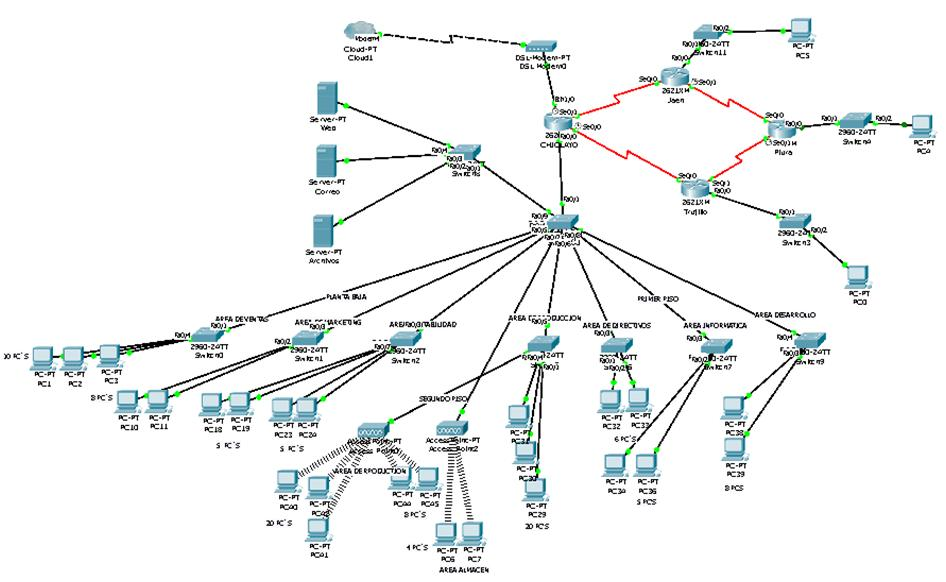
\includegraphics[scale=0.6]{log}
    \centering \title{Figura 2: Diseño lógico de LifeSecur}
\end{figure}

\section{Seguridad de las conexiones al exterior}

Las únicas conexiones existentes desde los servidores de nuestra empresa hacia el exterior será a través de servicios de internet, dichas conexiones se protegerán ante accesos no autorizados, tomando medidas para asegurar la disponibilidad de la conexión, dichas medidas serán las siguientes:

\begin{itemize}
\item \textbf{Seguridad mediante cortafuegos:} El principio de los mecanismos de seguridad de los sistemas corporativos es el de mantener a los intrusos fuera de la red de la empresa, permitiéndole a ésta realizar su trabajo.\\
La tecnología fundamental utilizada en estos casos es la instalación de un firewall o cortafuegos. En el entorno de redes de ordenadores, un cortafuegos es un sistema de contención que intenta impedir la diseminación de daños a través suyo. Físicamente, un cortafuegos de Internet es un sistema o grupo de sistemas informáticos situados en el perímetro de la red para proteger todas sus vías de acceso estableciendo un control del tráfico de entrada y salida. Por consiguiente, un cortafuegos sólo protege contra la diseminación de los ataques derivados de accesos públicos, es decir, sólo puede controlar el tráfico que pasa a través de él.
\item \textbf{Pasarelas a nivel de red:} Los cortafuegos más sencillos se basan en el filtrado de paquetes. Los dispositivos típicamente utilizados son los encaminadores apantallados, capaces de filtrar paquetes en base a la dirección origen y/o destino y al servicio o puerto al que acceden.\\
Se usará el filtrado para bloquear conexiones a o desde servidores o redes determinadas, así como para bloquear puertos especiales. Esto nos permite activar o desactivar servicios bien conocidos de forma selectiva para aquellos servidores o redes que no consideremos seguros o que queramos proteger especialmente.
\item \textbf{Pasarelas a nivel de aplicación:} Como hemos visto, los filtros de paquetes son demasiado rígidos, difíciles de configurar y sus capacidades de registro histórico son muy limitadas. Además, su funcionamiento de basa en un sistema todo o nada: el acceso a un servicio en o desde una máquina se permite o no, pero no hay un término medio.\\
El siguiente paso es usar pasarelas a nivel de aplicación (gateway o proxy): en estos sistemas el usuario no accede directamente al servicio sino un sistema intermedio que realiza las comprobaciones pertinentes anota la transacción, toma una decisión y, si es positiva, actúa de intermediario entre el cliente y el servicio remoto correspondiente, posiblemente controlando la ejecución del protocolo del servicio y tomando notas adicionales.
\item \textbf{Pasarelas de intercambio seguro:} Las pasarelas de intercambio seguro de información son dispositivos de protección de perímetro más complejos que un cortafuegos o un proxy. Están orientadas a la protección de interconexiones entre redes que manejan información con diferentes categorías o políticas de seguridad, con el fin de evitar la entrada o salida de información no autorizada.\\
Para ello, aportan las siguientes funcionalidades de seguridad:\\
\begin{itemize}
\item Separación de redes: Ruptura de la continuidad de los protocolos de comunicaciones entre dos redes interconectadas en todas las capas del modelo OSI.
\item Filtrado de contenidos: Las pasarelas analizan el contenido del paquete y permiten el paso de información siempre que cumpla las reglas de filtrado definidas, tanto para la entrada como para la salida.
\item Las pasarelas son especialmente útiles para implementar mecanismos de defensa en profundidad y neutralizar o minimizar el efecto de las Amenazas Persistentes Avanzadas al no permitir la fuga de información sensible desde la red interna.
\end{itemize}
\item \textbf{Diodos de datos:} Los diodos de datos son los dispositivos de protección de perímetro que aportan una mayor seguridad frente a la fuga de información sensible, dado que garantizan el flujo unidireccional de la información mediante hardware, al no existir un canal de retorno físico. 
\end{itemize}

\section{Seguridad de la información transmitida}

Las medidas para evitar que la información transmitida sea bloqueada,interceptada, modificada o falsamente fabricada son las siguientes:

\begin{itemize}
\item \textbf{Sistema operativo:} vamos a elegir el sistema operativo que es menos propenso a ataques, ya sea porque es menos utilizado en el mercado, o porque es el que menos vulnerabilidades presenta así evitando los ataques realizados a nuestra empresa.
\item \textbf{Navegador web:} Usaremos Mozilla Firefox ya que es un navegador superior a Internet Explorer de Microsoft. Mozilla tiende a "parchear" las vulnerabilidades de seguridad de Firefox con mayor frecuencia que Microsoft. Una de las ventajas de Firefox es que es un programa de "código abierto". Esto permite que nuestros profesionales de seguridad participen más en arreglar errores y crear funciones más fuertes de seguridad. Otra ventaja de Firefox es que cuenta con los "Add-Ons" que se pueden utilizar para fortalecer las funciones de privacidad de seguridad de Firefox.
\item \textbf{El uso de firewalls, programas antivirus y programas maliciosos:} Todos nuestros empleados deben estar familiarizados con los firewalls, programas antivirus y programas maliciosos. Estos programas trabajan en conjunto y deben utilizarse para proveer el máximo nivel de seguridad para proteger nuestros sistemas. Son necesarios para protegernos de amenazas que tienen como fin dañar, frustrar o infligir actividad ilegítima en nuestros sistemas.
\item \textbf{Uso de cuentas estándar o de acceso limitado:} Estas cuenta limitadas es para personas que tienen prohibido cambiar las configuraciones de la computadora y borrar archivos importantes. Un usuario con una cuenta limitada generalmente no puede instalar software o hardware. Sin embargo, puede acceder programas que ya fueron instalados en la computadora. Por otra parte, la cuenta del administrador es para alguien que tiene permitido hacer cambios en la computadora e instalar software.
\item \textbf{Mantener el software actualizado:} Los hackers siempre están buscando maneras nuevas de penetrar las defensas de los programas de software de los sistemas. Las compañías de software responden con parches para cerrar esas fallas de seguridad. Para mantenerse protegido, necesitamos descargar e instalar los parches tanto para nuestro sistema operativo como las aplicaciones de software cada vez que estén disponibles. Los parches de software o las actualizaciones generalmente solucionan los problemas o vulnerabilidades de un programa.
\item \textbf{Uso de contraseñas seguras y distintas:} Las contraseñas generalmente es lo único que protege la información privada. Sin embargo, muchos sitios se están haciendo más vulnerables porque frecuentemente se utilizan las mismas contraseñas en muchos sitios.
\item \textbf{Apagar la computadora o desconéctarla de Internet:}Si no se está utilizando la computadora por un periodo largo de tiempo, lo mejor es apagarla. Los módems de cable y las líneas DSL permite que las computadoras estén conectadas en todo momento. Esto es conveniente. Sin embargo, tiene varios riesgos. La probabilidad de que la computadora esté expuesta a estos riesgos es mucho más alta si la computadora siempre está conectada al Internet.
\end{itemize}

\section{Seguridad en el teletrabajo}

El personal que realice teletrabajo, tendrá que hacer constancia de su horario de trabajo mediante la web de la empresa, si  esta no está disponible se realizaría vía teléfono, identificándose como trabajador de la empresa autorizado de este tipo de trabajo.  

El acceso a los fichero deberá ser con permiso del responsable de seguridad informática y dejando constancia de la fecha, hora y datos para localizar la máquina y su propietario. 

Los archivos subidos dejaran también un registro, y deberán ser analizados con antivirus previa y posteriormente a su subida. 



\chapter{Política de continuidad del negocio}


\section{Ámbito}

Con continuidad del negocio nos referimos a todos aquellos mecanismos generalmente de recuperación, destinados a mantener la línea de trabajo del negoción sin generar ningún tipo de perdida de información, software y configuración del mismo. Por lo que este apartado de la política se aplica a toda la información, software y hardware.

\section{Objetivos}

El principal propósito de esta política es garantizar que no se pierda ninguna información, configuración de un software o equipo. Para así poder seguir ejecutando un trabajo continuado sin generar ningún tipo de pérdida económica o temporal al organismo. 

\section{Alcance y responsabilidades}

Esta política se aplica a toda la información, software y equipo hardware que contenga estas anteriores.

El responsable de seguridad será el responsable de las copias de seguridad del servidor, y de generar un procedimiento, mediante el que restablecer todos los datos mediante copias de seguridad.

Cada empleado será el responsable de guardar la configuración del software que utiliza, por si fuera necesario reestablecerlo en un futuro. 

\section{Continuidad de la actividad de la empresa}

La parte especialmente vital para el continuado funcionamiento de la organización, son el hardware y los datos alojados en el servidor, ya que contiene toda la información de los clientes. Y refiriéndonos a los datos, son más importante los de carácter sensible. Por lo que al restaurar la información, se recuperara primero la información del servidor, y dentro de esta la información de carácter sensible. Antes de restaurar la información repondríamos el hardware dañado. 

\section{Copias de seguridad}
\label{sec:copias-de-seguridad}

Las copias de seguridad que se realizaran será de toda la información del servidor, cada mes. La configuración del servidor y los cortafuegos, cada vez que en esta configuración se realice  algún tipo de cambio.

En las estaciones de trabajo deberá realizarse copia de seguridad de la configuración del software, si se ha realizado muchos cambios, con el mismo periodo que los servidores. De esta manera garantizamos agilidad a la hora de volver al trabajo en una recuperación.

Los datos de la estaciones de trabajo no deberíamos de hacer copias de seguridad, ya que al terminar la jornada laboral deberán ser subidos al servidor. 

\section{Recuperación de activos}
\label{sec:desastre}

La planificación para la recuperación de un activo sería primeramente restaurar el hardware dañado o que esté dando fallos. Luego se restauraría la información como hemos definido en el apartado anterior. Una vez se restablezca la información del servidor, procedería restaurar la configuración tanto del servidor como del cortafuegos y los equipos del personal.

Un empleado del departamento de seguridad es el responsable de mantener la documentación actualizada sobre el estado de la configuración de los sistemas.


\appendix

\chapter{Presupuestos de material}
Aquí se listará una serie de presupuestos iniciales para los
distintos elementos que puedan utilizarse para llevar a cabo la
política.

\section{Software}

Presupuestos del software necesario: cortafuegos, antivirus, etc.

\section{Hardware}

Presupuestos del hardware necesario: equipamiento de red, sistemas de
alimentación ininterrumpida, etc.

\section{Infraestructuras}

Presupuestos para los materiales de infraestructuras: detectores de
humo, detectores de presencia, cámaras de seguridad, armarios
ignífugos, cerrojos de múltiples cilindros, extintores, etc.

\section{Servicios}

Presupuestos para cursos de formación y concienciación (a menos que
sean internos), contratación de personal de seguridad, alquiler de
cámaras conectadas a una centralita remota, etc.


\chapter{Otros anexos}

Se dedicarán más anexos para aquellas listas y materiales que por su
extensión rompan el flujo normal del texto de una determinada
política, o que se consideren que pueden cambiar con más frecuencia.

Posibles anexos incluyen:

\begin{itemize}
\item Formularios a utilizar para gestionar las incidencias
\item Normativa y legislación aplicable
\item Procedimientos del responsable de seguridad y/o el comité de seguridad
\end{itemize}

\chapter{Anexo C. Formulario de solicitud de cambio}

El formulario de solicitud de cambio solo podrá ser rellenado por los empleados de la organización.

Una vez completado, el empleado debe transmitir dicho formulario al responsable del departamento del área al que pertenezca, y será transmitido vía e-mail o físicamente. Este formulario será, posteriormente, evaluado por el responsable de seguridad. Será este el que determine su aprobación y entrada en vigor.


%%

\backmatter
\bibliographystyle{hispa}
\bibliography{bibliografia.bib}

\end{document}

%%% Local Variables: 
%%% mode: latex
%%% TeX-master: t
%%% End: 
